\chapter{Range queries}

\index{range query}
\index{sum query}
\index{minimum query}
\index{maximum query}

In this chapter, we discuss data structures
that allow us to efficiently process range queries.
In a \key{range query},
our task is to calculate a value
based on a subarray of an array.
Typical range queries are:
\begin{itemize}
\item $\texttt{sum}_q(a,b)$: calculate the sum of values in range $[a,b]$
\item $\texttt{min}_q(a,b)$: find the minimum value in range $[a,b]$
\item $\texttt{max}_q(a,b)$: find the maximum value in range $[a,b]$
\end{itemize}

For example, consider the range $[3,6]$ in the following array:
\begin{center}
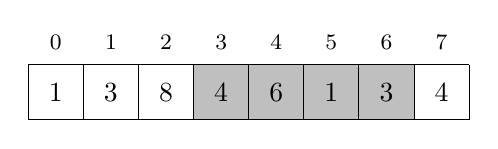
\begin{tikzpicture}[scale=0.7]
\fill[color=lightgray] (3,0) rectangle (7,1);
\draw (0,0) grid (8,1);

\node at (0.5,0.5) {$1$};
\node at (1.5,0.5) {$3$};
\node at (2.5,0.5) {$8$};
\node at (3.5,0.5) {$4$};
\node at (4.5,0.5) {$6$};
\node at (5.5,0.5) {$1$};
\node at (6.5,0.5) {$3$};
\node at (7.5,0.5) {$4$};

\footnotesize
\node at (0.5,1.4) {$0$};
\node at (1.5,1.4) {$1$};
\node at (2.5,1.4) {$2$};
\node at (3.5,1.4) {$3$};
\node at (4.5,1.4) {$4$};
\node at (5.5,1.4) {$5$};
\node at (6.5,1.4) {$6$};
\node at (7.5,1.4) {$7$};
\end{tikzpicture}
\end{center}
In this case, $\texttt{sum}_q(3,6)=14$,
$\texttt{min}_q(3,6)=1$ and $\texttt{max}_q(3,6)=6$.

A simple way to process range queries is to use
a loop that goes through all array values in the range.
For example, the following function can be
used to process sum queries on an array:

\begin{lstlisting}
int sum(int a, int b) {
    int s = 0;
    for (int i = a; i <= b; i++) {
        s += array[i];
    }
    return s;
}
\end{lstlisting}

This function works in $O(n)$ time,
where $n$ is the size of the array.
Thus, we can process $q$ queries in $O(nq)$
time using the function.
However, if both $n$ and $q$ are large, this approach
is slow. Fortunately, it turns out that there are
ways to process range queries much more efficiently.

\section{Static array queries}

We first focus on a situation where
the array is \emph{static}, i.e.,
the array values are never updated between the queries.
In this case, it suffices to construct
a static data structure that tells us
the answer for any possible query.

\subsubsection{Sum queries}

\index{prefix sum array}

We can easily process
sum queries on a static array
by constructing a \key{prefix sum array}.
Each value in the prefix sum array equals
the sum of values in the original array up to that position,
i.e., the value at position $k$ is $\texttt{sum}_q(0,k)$.
The prefix sum array can be constructed in $O(n)$ time.

For example, consider the following array:
\begin{center}
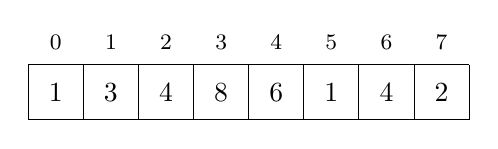
\begin{tikzpicture}[scale=0.7]
%\fill[color=lightgray] (3,0) rectangle (7,1);
\draw (0,0) grid (8,1);

\node at (0.5,0.5) {$1$};
\node at (1.5,0.5) {$3$};
\node at (2.5,0.5) {$4$};
\node at (3.5,0.5) {$8$};
\node at (4.5,0.5) {$6$};
\node at (5.5,0.5) {$1$};
\node at (6.5,0.5) {$4$};
\node at (7.5,0.5) {$2$};

\footnotesize
\node at (0.5,1.4) {$0$};
\node at (1.5,1.4) {$1$};
\node at (2.5,1.4) {$2$};
\node at (3.5,1.4) {$3$};
\node at (4.5,1.4) {$4$};
\node at (5.5,1.4) {$5$};
\node at (6.5,1.4) {$6$};
\node at (7.5,1.4) {$7$};
\end{tikzpicture}
\end{center}
The corresponding prefix sum array is as follows:
\begin{center}
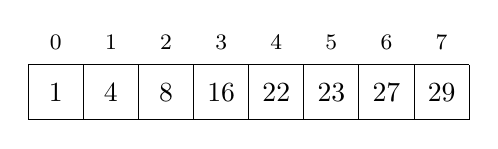
\begin{tikzpicture}[scale=0.7]
%\fill[color=lightgray] (3,0) rectangle (7,1);
\draw (0,0) grid (8,1);

\node at (0.5,0.5) {$1$};
\node at (1.5,0.5) {$4$};
\node at (2.5,0.5) {$8$};
\node at (3.5,0.5) {$16$};
\node at (4.5,0.5) {$22$};
\node at (5.5,0.5) {$23$};
\node at (6.5,0.5) {$27$};
\node at (7.5,0.5) {$29$};


\footnotesize
\node at (0.5,1.4) {$0$};
\node at (1.5,1.4) {$1$};
\node at (2.5,1.4) {$2$};
\node at (3.5,1.4) {$3$};
\node at (4.5,1.4) {$4$};
\node at (5.5,1.4) {$5$};
\node at (6.5,1.4) {$6$};
\node at (7.5,1.4) {$7$};
\end{tikzpicture}
\end{center}
Since the prefix sum array contains all values
of $\texttt{sum}_q(0,k)$,
we can calculate any value of
$\texttt{sum}_q(a,b)$ in $O(1)$ time as follows:
\[ \texttt{sum}_q(a,b) = \texttt{sum}_q(0,b) - \texttt{sum}_q(0,a-1)\]
By defining $\texttt{sum}_q(0,-1)=0$,
the above formula also holds when $a=0$.

For example, consider the range $[3,6]$:
\begin{center}
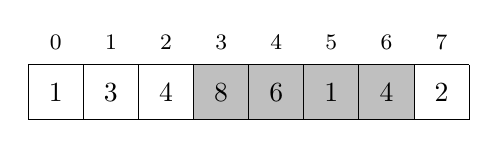
\begin{tikzpicture}[scale=0.7]
\fill[color=lightgray] (3,0) rectangle (7,1);
\draw (0,0) grid (8,1);

\node at (0.5,0.5) {$1$};
\node at (1.5,0.5) {$3$};
\node at (2.5,0.5) {$4$};
\node at (3.5,0.5) {$8$};
\node at (4.5,0.5) {$6$};
\node at (5.5,0.5) {$1$};
\node at (6.5,0.5) {$4$};
\node at (7.5,0.5) {$2$};

\footnotesize
\node at (0.5,1.4) {$0$};
\node at (1.5,1.4) {$1$};
\node at (2.5,1.4) {$2$};
\node at (3.5,1.4) {$3$};
\node at (4.5,1.4) {$4$};
\node at (5.5,1.4) {$5$};
\node at (6.5,1.4) {$6$};
\node at (7.5,1.4) {$7$};
\end{tikzpicture}
\end{center}
In this case $\texttt{sum}_q(3,6)=8+6+1+4=19$.
This sum can be calculated from
two values of the prefix sum array:
\begin{center}
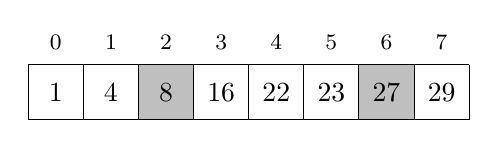
\begin{tikzpicture}[scale=0.7]
\fill[color=lightgray] (2,0) rectangle (3,1);
\fill[color=lightgray] (6,0) rectangle (7,1);
\draw (0,0) grid (8,1);

\node at (0.5,0.5) {$1$};
\node at (1.5,0.5) {$4$};
\node at (2.5,0.5) {$8$};
\node at (3.5,0.5) {$16$};
\node at (4.5,0.5) {$22$};
\node at (5.5,0.5) {$23$};
\node at (6.5,0.5) {$27$};
\node at (7.5,0.5) {$29$};

\footnotesize
\node at (0.5,1.4) {$0$};
\node at (1.5,1.4) {$1$};
\node at (2.5,1.4) {$2$};
\node at (3.5,1.4) {$3$};
\node at (4.5,1.4) {$4$};
\node at (5.5,1.4) {$5$};
\node at (6.5,1.4) {$6$};
\node at (7.5,1.4) {$7$};
\end{tikzpicture}
\end{center}
Thus, $\texttt{sum}_q(3,6)=\texttt{sum}_q(0,6)-\texttt{sum}_q(0,2)=27-8=19$.

It is also possible to generalize this idea
to higher dimensions.
For example, we can construct a two-dimensional
prefix sum array that can be used to calculate
the sum of any rectangular subarray in $O(1)$ time.
Each sum in such an array corresponds to
a subarray
that begins at the upper-left corner of the array.

\begin{samepage}
The following picture illustrates the idea:
\begin{center}
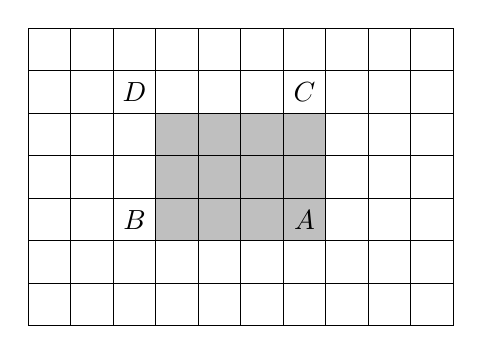
\begin{tikzpicture}[scale=0.54]
\draw[fill=lightgray] (3,2) rectangle (7,5);
\draw (0,0) grid (10,7);
\node[anchor=center] at (6.5, 2.5) {$A$};
\node[anchor=center] at (2.5, 2.5) {$B$};
\node[anchor=center] at (6.5, 5.5) {$C$};
\node[anchor=center] at (2.5, 5.5) {$D$};
\end{tikzpicture}
\end{center}
\end{samepage}

The sum of the gray subarray can be calculated
using the formula
\[S(A) - S(B) - S(C) + S(D),\]
where $S(X)$ denotes the sum of values
in a rectangular
subarray from the upper-left corner
to the position of $X$.

\subsubsection{Minimum queries}

\index{sparse table}

Minimum queries are more difficult to process
than sum queries.
Still, there is a quite simple 
$O(n \log n)$ time preprocessing
method after which we can answer any minimum
query in $O(1)$ time\footnote{This technique
was introduced in \cite{ben00} and sometimes
called the \key{sparse table} method.
There are also more sophisticated techniques \cite{fis06} where
the preprocessing time is only $O(n)$, but such algorithms
are not needed in competitive programming.}.
Note that since minimum and maximum queries can
be processed similarly,
we can focus on minimum queries.

The idea is to precalculate all values of
$\textrm{min}_q(a,b)$ where
$b-a+1$ (the length of the range) is a power of two.
For example, for the array

\begin{center}
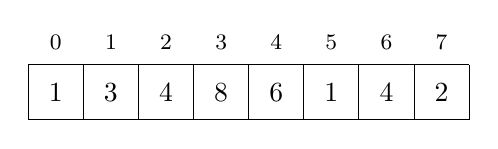
\begin{tikzpicture}[scale=0.7]
\draw (0,0) grid (8,1);

\node at (0.5,0.5) {$1$};
\node at (1.5,0.5) {$3$};
\node at (2.5,0.5) {$4$};
\node at (3.5,0.5) {$8$};
\node at (4.5,0.5) {$6$};
\node at (5.5,0.5) {$1$};
\node at (6.5,0.5) {$4$};
\node at (7.5,0.5) {$2$};

\footnotesize
\node at (0.5,1.4) {$0$};
\node at (1.5,1.4) {$1$};
\node at (2.5,1.4) {$2$};
\node at (3.5,1.4) {$3$};
\node at (4.5,1.4) {$4$};
\node at (5.5,1.4) {$5$};
\node at (6.5,1.4) {$6$};
\node at (7.5,1.4) {$7$};
\end{tikzpicture}
\end{center}
the following values are calculated:

\begin{center}
\begin{tabular}{ccc}

\begin{tabular}{lll}
$a$ & $b$ & $\texttt{min}_q(a,b)$ \\
\hline
0 & 0 & 1 \\
1 & 1 & 3 \\
2 & 2 & 4 \\
3 & 3 & 8 \\
4 & 4 & 6 \\
5 & 5 & 1 \\
6 & 6 & 4 \\
7 & 7 & 2 \\
\end{tabular}

&

\begin{tabular}{lll}
$a$ & $b$ & $\texttt{min}_q(a,b)$ \\
\hline
0 & 1 & 1 \\
1 & 2 & 3 \\
2 & 3 & 4 \\
3 & 4 & 6 \\
4 & 5 & 1 \\
5 & 6 & 1 \\
6 & 7 & 2 \\
\\
\end{tabular}

&

\begin{tabular}{lll}
$a$ & $b$ & $\texttt{min}_q(a,b)$ \\
\hline
0 & 3 & 1 \\
1 & 4 & 3 \\
2 & 5 & 1 \\
3 & 6 & 1 \\
4 & 7 & 1 \\
0 & 7 & 1 \\
\\
\\
\end{tabular}

\end{tabular}
\end{center}

The number of precalculated values is $O(n \log n)$,
because there are $O(\log n)$ range lengths
that are powers of two.
The values can be calculated efficiently
using the recursive formula
\[\texttt{min}_q(a,b) = \min(\texttt{min}_q(a,a+w-1),\texttt{min}_q(a+w,b)),\]
where $b-a+1$ is a power of two and $w=(b-a+1)/2$.
Calculating all those values takes $O(n \log n)$ time.

After this, any value of $\texttt{min}_q(a,b)$ can be calculated
in $O(1)$ time as a minimum of two precalculated values.
Let $k$ be the largest power of two that does not exceed $b-a+1$.
We can calculate the value of $\texttt{min}_q(a,b)$ using the formula
\[\texttt{min}_q(a,b) = \min(\texttt{min}_q(a,a+k-1),\texttt{min}_q(b-k+1,b)).\]
In the above formula, the range $[a,b]$ is represented
as the union of the ranges $[a,a+k-1]$ and $[b-k+1,b]$, both of length $k$.

As an example, consider the range $[1,6]$:
\begin{center}
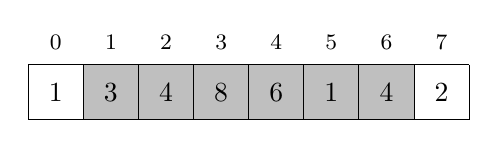
\begin{tikzpicture}[scale=0.7]
\fill[color=lightgray] (1,0) rectangle (7,1);
\draw (0,0) grid (8,1);

\node at (0.5,0.5) {$1$};
\node at (1.5,0.5) {$3$};
\node at (2.5,0.5) {$4$};
\node at (3.5,0.5) {$8$};
\node at (4.5,0.5) {$6$};
\node at (5.5,0.5) {$1$};
\node at (6.5,0.5) {$4$};
\node at (7.5,0.5) {$2$};

\footnotesize
\node at (0.5,1.4) {$0$};
\node at (1.5,1.4) {$1$};
\node at (2.5,1.4) {$2$};
\node at (3.5,1.4) {$3$};
\node at (4.5,1.4) {$4$};
\node at (5.5,1.4) {$5$};
\node at (6.5,1.4) {$6$};
\node at (7.5,1.4) {$7$};
\end{tikzpicture}
\end{center}
The length of the range is 6,
and the largest power of two that does
not exceed 6 is 4.
Thus the range $[1,6]$ is
the union of the ranges $[1,4]$ and $[3,6]$:
\begin{center}
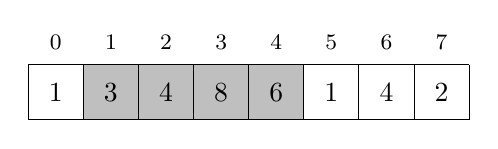
\begin{tikzpicture}[scale=0.7]
\fill[color=lightgray] (1,0) rectangle (5,1);
\draw (0,0) grid (8,1);

\node at (0.5,0.5) {$1$};
\node at (1.5,0.5) {$3$};
\node at (2.5,0.5) {$4$};
\node at (3.5,0.5) {$8$};
\node at (4.5,0.5) {$6$};
\node at (5.5,0.5) {$1$};
\node at (6.5,0.5) {$4$};
\node at (7.5,0.5) {$2$};

\footnotesize
\node at (0.5,1.4) {$0$};
\node at (1.5,1.4) {$1$};
\node at (2.5,1.4) {$2$};
\node at (3.5,1.4) {$3$};
\node at (4.5,1.4) {$4$};
\node at (5.5,1.4) {$5$};
\node at (6.5,1.4) {$6$};
\node at (7.5,1.4) {$7$};
\end{tikzpicture}
\end{center}
\begin{center}
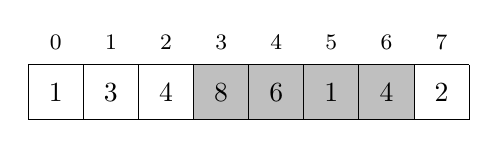
\begin{tikzpicture}[scale=0.7]
\fill[color=lightgray] (3,0) rectangle (7,1);
\draw (0,0) grid (8,1);

\node at (0.5,0.5) {$1$};
\node at (1.5,0.5) {$3$};
\node at (2.5,0.5) {$4$};
\node at (3.5,0.5) {$8$};
\node at (4.5,0.5) {$6$};
\node at (5.5,0.5) {$1$};
\node at (6.5,0.5) {$4$};
\node at (7.5,0.5) {$2$};


\footnotesize
\node at (0.5,1.4) {$0$};
\node at (1.5,1.4) {$1$};
\node at (2.5,1.4) {$2$};
\node at (3.5,1.4) {$3$};
\node at (4.5,1.4) {$4$};
\node at (5.5,1.4) {$5$};
\node at (6.5,1.4) {$6$};
\node at (7.5,1.4) {$7$};
\end{tikzpicture}
\end{center}
Since $\texttt{min}_q(1,4)=3$ and $\texttt{min}_q(3,6)=1$,
we conclude that $\texttt{min}_q(1,6)=1$.

\section{Binary indexed tree}

\index{binary indexed tree}
\index{Fenwick tree}

A \key{binary indexed tree} or a \key{Fenwick tree}\footnote{The
binary indexed tree structure was presented by P. M. Fenwick in 1994 \cite{fen94}.}
can be seen as a dynamic variant of a prefix sum array.
It supports two $O(\log n)$ time operations on an array:
processing a range sum query and updating a value.

The advantage of a binary indexed tree is
that it allows us to efficiently update
array values between sum queries.
This would not be possible using a prefix sum array,
because after each update, it would be necessary to build the
whole prefix sum array again in $O(n)$ time.

\subsubsection{Structure}

Even if the name of the structure is a binary indexed \emph{tree},
it is usually represented as an array.
In this section we assume that all arrays are one-indexed,
because it makes the implementation easier.

Let $p(k)$ denote the largest power of two that
divides $k$.
We store a binary indexed tree as an array \texttt{tree}
such that
\[ \texttt{tree}[k] = \texttt{sum}_q(k-p(k)+1,k),\]
i.e., each position $k$ contains the sum of values
in a range of the original array whose length is $p(k)$
and that ends at position $k$.
For example, since $p(6)=2$, $\texttt{tree}[6]$
contains the value of $\texttt{sum}_q(5,6)$.

For example, consider the following array:
\begin{center}
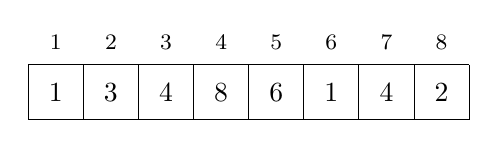
\begin{tikzpicture}[scale=0.7]
\draw (0,0) grid (8,1);

\node at (0.5,0.5) {$1$};
\node at (1.5,0.5) {$3$};
\node at (2.5,0.5) {$4$};
\node at (3.5,0.5) {$8$};
\node at (4.5,0.5) {$6$};
\node at (5.5,0.5) {$1$};
\node at (6.5,0.5) {$4$};
\node at (7.5,0.5) {$2$};

\footnotesize
\node at (0.5,1.4) {$1$};
\node at (1.5,1.4) {$2$};
\node at (2.5,1.4) {$3$};
\node at (3.5,1.4) {$4$};
\node at (4.5,1.4) {$5$};
\node at (5.5,1.4) {$6$};
\node at (6.5,1.4) {$7$};
\node at (7.5,1.4) {$8$};
\end{tikzpicture}
\end{center}

The corresponding binary indexed tree is as follows:
\begin{center}
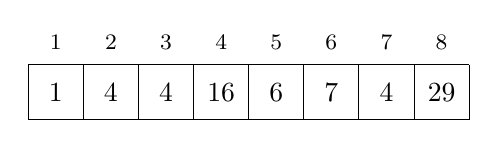
\begin{tikzpicture}[scale=0.7]
\draw (0,0) grid (8,1);

\node at (0.5,0.5) {$1$};
\node at (1.5,0.5) {$4$};
\node at (2.5,0.5) {$4$};
\node at (3.5,0.5) {$16$};
\node at (4.5,0.5) {$6$};
\node at (5.5,0.5) {$7$};
\node at (6.5,0.5) {$4$};
\node at (7.5,0.5) {$29$};

\footnotesize
\node at (0.5,1.4) {$1$};
\node at (1.5,1.4) {$2$};
\node at (2.5,1.4) {$3$};
\node at (3.5,1.4) {$4$};
\node at (4.5,1.4) {$5$};
\node at (5.5,1.4) {$6$};
\node at (6.5,1.4) {$7$};
\node at (7.5,1.4) {$8$};
\end{tikzpicture}
\end{center}

The following picture shows more clearly
how each value in the binary indexed tree
corresponds to a range in the original array:

\begin{center}
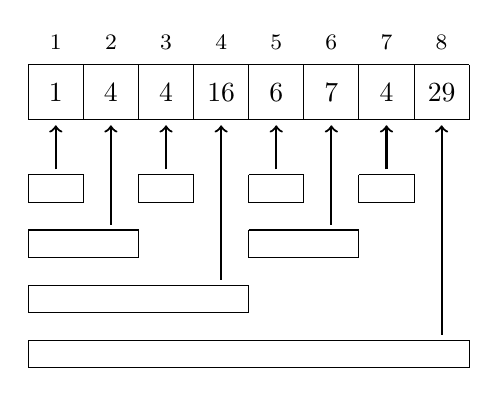
\begin{tikzpicture}[scale=0.7]
\draw (0,0) grid (8,1);

\node at (0.5,0.5) {$1$};
\node at (1.5,0.5) {$4$};
\node at (2.5,0.5) {$4$};
\node at (3.5,0.5) {$16$};
\node at (4.5,0.5) {$6$};
\node at (5.5,0.5) {$7$};
\node at (6.5,0.5) {$4$};
\node at (7.5,0.5) {$29$};

\footnotesize
\node at (0.5,1.4) {$1$};
\node at (1.5,1.4) {$2$};
\node at (2.5,1.4) {$3$};
\node at (3.5,1.4) {$4$};
\node at (4.5,1.4) {$5$};
\node at (5.5,1.4) {$6$};
\node at (6.5,1.4) {$7$};
\node at (7.5,1.4) {$8$};

\draw[->,thick] (0.5,-0.9) -- (0.5,-0.1);
\draw[->,thick] (2.5,-0.9) -- (2.5,-0.1);
\draw[->,thick] (4.5,-0.9) -- (4.5,-0.1);
\draw[->,thick] (6.5,-0.9) -- (6.5,-0.1);
\draw[->,thick] (1.5,-1.9) -- (1.5,-0.1);
\draw[->,thick] (5.5,-1.9) -- (5.5,-0.1);
\draw[->,thick] (3.5,-2.9) -- (3.5,-0.1);
\draw[->,thick] (7.5,-3.9) -- (7.5,-0.1);

\draw (0,-1) -- (1,-1) -- (1,-1.5) -- (0,-1.5) -- (0,-1);
\draw (2,-1) -- (3,-1) -- (3,-1.5) -- (2,-1.5) -- (2,-1);
\draw (4,-1) -- (5,-1) -- (5,-1.5) -- (4,-1.5) -- (4,-1);
\draw (6,-1) -- (7,-1) -- (7,-1.5) -- (6,-1.5) -- (6,-1);
\draw (0,-2) -- (2,-2) -- (2,-2.5) -- (0,-2.5) -- (0,-2);
\draw (4,-2) -- (6,-2) -- (6,-2.5) -- (4,-2.5) -- (4,-2);
\draw (0,-3) -- (4,-3) -- (4,-3.5) -- (0,-3.5) -- (0,-3);
\draw (0,-4) -- (8,-4) -- (8,-4.5) -- (0,-4.5) -- (0,-4);
\end{tikzpicture}
\end{center}

Using a binary indexed tree,
any value of $\texttt{sum}_q(1,k)$
can be calculated in $O(\log n)$ time,
because a range $[1,k]$ can always be divided into
$O(\log n)$ ranges whose sums are stored in the tree.

For example, the range $[1,7]$ consists of
the following ranges:
\begin{center}
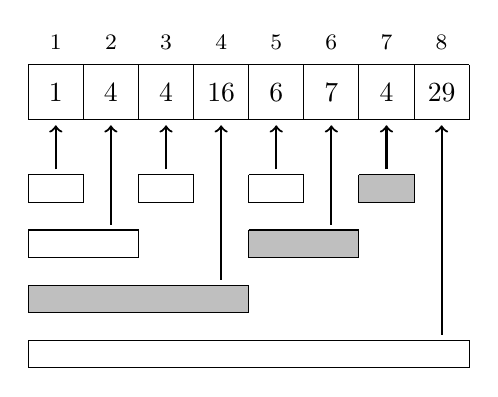
\begin{tikzpicture}[scale=0.7]
\draw (0,0) grid (8,1);

\node at (0.5,0.5) {$1$};
\node at (1.5,0.5) {$4$};
\node at (2.5,0.5) {$4$};
\node at (3.5,0.5) {$16$};
\node at (4.5,0.5) {$6$};
\node at (5.5,0.5) {$7$};
\node at (6.5,0.5) {$4$};
\node at (7.5,0.5) {$29$};

\footnotesize
\node at (0.5,1.4) {$1$};
\node at (1.5,1.4) {$2$};
\node at (2.5,1.4) {$3$};
\node at (3.5,1.4) {$4$};
\node at (4.5,1.4) {$5$};
\node at (5.5,1.4) {$6$};
\node at (6.5,1.4) {$7$};
\node at (7.5,1.4) {$8$};

\draw[->,thick] (0.5,-0.9) -- (0.5,-0.1);
\draw[->,thick] (2.5,-0.9) -- (2.5,-0.1);
\draw[->,thick] (4.5,-0.9) -- (4.5,-0.1);
\draw[->,thick] (6.5,-0.9) -- (6.5,-0.1);
\draw[->,thick] (1.5,-1.9) -- (1.5,-0.1);
\draw[->,thick] (5.5,-1.9) -- (5.5,-0.1);
\draw[->,thick] (3.5,-2.9) -- (3.5,-0.1);
\draw[->,thick] (7.5,-3.9) -- (7.5,-0.1);

\draw (0,-1) -- (1,-1) -- (1,-1.5) -- (0,-1.5) -- (0,-1);
\draw (2,-1) -- (3,-1) -- (3,-1.5) -- (2,-1.5) -- (2,-1);
\draw (4,-1) -- (5,-1) -- (5,-1.5) -- (4,-1.5) -- (4,-1);
\draw[fill=lightgray] (6,-1) -- (7,-1) -- (7,-1.5) -- (6,-1.5) -- (6,-1);
\draw (0,-2) -- (2,-2) -- (2,-2.5) -- (0,-2.5) -- (0,-2);
\draw[fill=lightgray] (4,-2) -- (6,-2) -- (6,-2.5) -- (4,-2.5) -- (4,-2);
\draw[fill=lightgray] (0,-3) -- (4,-3) -- (4,-3.5) -- (0,-3.5) -- (0,-3);
\draw (0,-4) -- (8,-4) -- (8,-4.5) -- (0,-4.5) -- (0,-4);
\end{tikzpicture}
\end{center}
Thus, we can calculate the corresponding sum as follows:
\[\texttt{sum}_q(1,7)=\texttt{sum}_q(1,4)+\texttt{sum}_q(5,6)+\texttt{sum}_q(7,7)=16+7+4=27\]

To calculate the value of $\texttt{sum}_q(a,b)$ where $a>1$,
we can use the same trick that we used with prefix sum arrays:
\[ \texttt{sum}_q(a,b) = \texttt{sum}_q(1,b) - \texttt{sum}_q(1,a-1).\]
Since we can calculate both $\texttt{sum}_q(1,b)$
and $\texttt{sum}_q(1,a-1)$ in $O(\log n)$ time,
the total time complexity is $O(\log n)$.

Then, after updating a value in the original array,
several values in the binary indexed tree
should be updated.
For example, if the value at position 3 changes,
the sums of the following ranges change:
\begin{center}
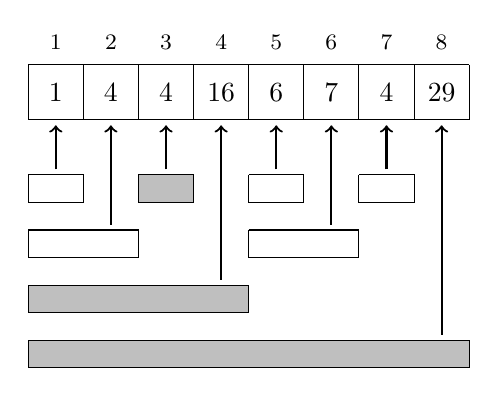
\begin{tikzpicture}[scale=0.7]
\draw (0,0) grid (8,1);

\node at (0.5,0.5) {$1$};
\node at (1.5,0.5) {$4$};
\node at (2.5,0.5) {$4$};
\node at (3.5,0.5) {$16$};
\node at (4.5,0.5) {$6$};
\node at (5.5,0.5) {$7$};
\node at (6.5,0.5) {$4$};
\node at (7.5,0.5) {$29$};

\footnotesize
\node at (0.5,1.4) {$1$};
\node at (1.5,1.4) {$2$};
\node at (2.5,1.4) {$3$};
\node at (3.5,1.4) {$4$};
\node at (4.5,1.4) {$5$};
\node at (5.5,1.4) {$6$};
\node at (6.5,1.4) {$7$};
\node at (7.5,1.4) {$8$};

\draw[->,thick] (0.5,-0.9) -- (0.5,-0.1);
\draw[->,thick] (2.5,-0.9) -- (2.5,-0.1);
\draw[->,thick] (4.5,-0.9) -- (4.5,-0.1);
\draw[->,thick] (6.5,-0.9) -- (6.5,-0.1);
\draw[->,thick] (1.5,-1.9) -- (1.5,-0.1);
\draw[->,thick] (5.5,-1.9) -- (5.5,-0.1);
\draw[->,thick] (3.5,-2.9) -- (3.5,-0.1);
\draw[->,thick] (7.5,-3.9) -- (7.5,-0.1);

\draw (0,-1) -- (1,-1) -- (1,-1.5) -- (0,-1.5) -- (0,-1);
\draw[fill=lightgray] (2,-1) -- (3,-1) -- (3,-1.5) -- (2,-1.5) -- (2,-1);
\draw (4,-1) -- (5,-1) -- (5,-1.5) -- (4,-1.5) -- (4,-1);
\draw (6,-1) -- (7,-1) -- (7,-1.5) -- (6,-1.5) -- (6,-1);
\draw (0,-2) -- (2,-2) -- (2,-2.5) -- (0,-2.5) -- (0,-2);
\draw (4,-2) -- (6,-2) -- (6,-2.5) -- (4,-2.5) -- (4,-2);
\draw[fill=lightgray] (0,-3) -- (4,-3) -- (4,-3.5) -- (0,-3.5) -- (0,-3);
\draw[fill=lightgray] (0,-4) -- (8,-4) -- (8,-4.5) -- (0,-4.5) -- (0,-4);
\end{tikzpicture}
\end{center}

Since each array element belongs to $O(\log n)$
ranges in the binary indexed tree,
it suffices to update $O(\log n)$ values in the tree.

\subsubsection{Implementation}

The operations of a binary indexed tree can be
efficiently implemented using bit operations.
The key fact needed is that we can
calculate any value of $p(k)$ using the formula
\[p(k) = k \& -k.\]

The following function calculates the value of $\texttt{sum}_q(1,k)$:
\begin{lstlisting}
int sum(int k) {
    int s = 0;
    while (k >= 1) {
        s += tree[k];
        k -= k&-k;
    }
    return s;
}
\end{lstlisting}

The following function increases the
array value at position $k$ by $x$
($x$ can be positive or negative):
\begin{lstlisting}
void add(int k, int x) {
    while (k <= n) {
        tree[k] += x;
        k += k&-k;
    }
}
\end{lstlisting}

The time complexity of both the functions is
$O(\log n)$, because the functions access $O(\log n)$
values in the binary indexed tree, and each move
to the next position takes $O(1)$ time.

\section{Segment tree}

\index{segment tree}

A \key{segment tree}\footnote{The bottom-up-implementation in this chapter corresponds to
that in \cite{sta06}. Similar structures were used
in late 1970's to solve geometric problems \cite{ben80}.} is a data structure
that supports two operations:
processing a range query and
updating an array value.
Segment trees can support
sum queries, minimum and maximum queries and many other
queries so that both operations work in $O(\log n)$ time.

Compared to a binary indexed tree,
the advantage of a segment tree is that it is
a more general data structure.
While binary indexed trees only support
sum queries\footnote{In fact, using \emph{two} binary
indexed trees it is possible to support minimum queries \cite{dim15},
but this is more complicated than to use a segment tree.},
segment trees also support other queries.
On the other hand, a segment tree requires more
memory and is a bit more difficult to implement.

\subsubsection{Structure}

A segment tree is a binary tree
such that the nodes on the bottom level of the tree
correspond to the array elements,
and the other nodes
contain information needed for processing range queries.

In this section, we assume that the size
of the array is a power of two and zero-based
indexing is used, because it is convenient to build
a segment tree for such an array.
If the size of the array is not a power of two,
we can always append extra elements to it.

We will first discuss segment trees that support sum queries.
As an example, consider the following array:
\begin{center}
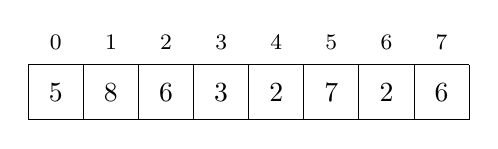
\begin{tikzpicture}[scale=0.7]
\draw (0,0) grid (8,1);

\node at (0.5,0.5) {$5$};
\node at (1.5,0.5) {$8$};
\node at (2.5,0.5) {$6$};
\node at (3.5,0.5) {$3$};
\node at (4.5,0.5) {$2$};
\node at (5.5,0.5) {$7$};
\node at (6.5,0.5) {$2$};
\node at (7.5,0.5) {$6$};

\footnotesize
\node at (0.5,1.4) {$0$};
\node at (1.5,1.4) {$1$};
\node at (2.5,1.4) {$2$};
\node at (3.5,1.4) {$3$};
\node at (4.5,1.4) {$4$};
\node at (5.5,1.4) {$5$};
\node at (6.5,1.4) {$6$};
\node at (7.5,1.4) {$7$};
\end{tikzpicture}
\end{center}
The corresponding segment tree is as follows:
\begin{center}
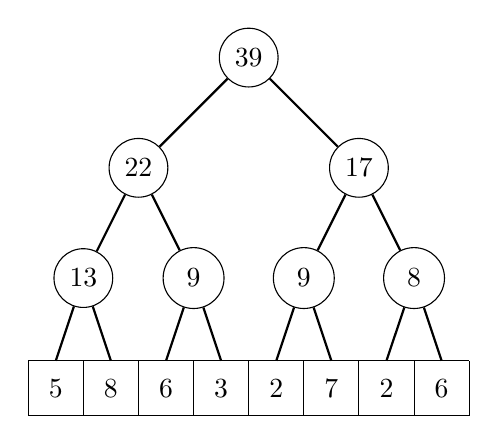
\begin{tikzpicture}[scale=0.7]
\draw (0,0) grid (8,1);

\node[anchor=center] at (0.5, 0.5) {5};
\node[anchor=center] at (1.5, 0.5) {8};
\node[anchor=center] at (2.5, 0.5) {6};
\node[anchor=center] at (3.5, 0.5) {3};
\node[anchor=center] at (4.5, 0.5) {2};
\node[anchor=center] at (5.5, 0.5) {7};
\node[anchor=center] at (6.5, 0.5) {2};
\node[anchor=center] at (7.5, 0.5) {6};

\node[draw, circle] (a) at (1,2.5) {13};
\path[draw,thick,-] (a) -- (0.5,1);
\path[draw,thick,-] (a) -- (1.5,1);
\node[draw, circle,minimum size=22pt] (b) at (3,2.5) {9};
\path[draw,thick,-] (b) -- (2.5,1);
\path[draw,thick,-] (b) -- (3.5,1);
\node[draw, circle,minimum size=22pt] (c) at (5,2.5) {9};
\path[draw,thick,-] (c) -- (4.5,1);
\path[draw,thick,-] (c) -- (5.5,1);
\node[draw, circle,minimum size=22pt] (d) at (7,2.5) {8};
\path[draw,thick,-] (d) -- (6.5,1);
\path[draw,thick,-] (d) -- (7.5,1);

\node[draw, circle] (i) at (2,4.5) {22};
\path[draw,thick,-] (i) -- (a);
\path[draw,thick,-] (i) -- (b);
\node[draw, circle] (j) at (6,4.5) {17};
\path[draw,thick,-] (j) -- (c);
\path[draw,thick,-] (j) -- (d);

\node[draw, circle] (m) at (4,6.5) {39};
\path[draw,thick,-] (m) -- (i);
\path[draw,thick,-] (m) -- (j);
\end{tikzpicture}
\end{center}

Each internal tree node
corresponds to an array range
whose size is a power of two.
In the above tree, the value of each internal
node is the sum of the corresponding array values,
and it can be calculated as the sum of
the values of its left and right child node.

It turns out that any range $[a,b]$
can be divided into $O(\log n)$ ranges
whose values are stored in tree nodes.
For example, consider the range [2,7]:
\begin{center}
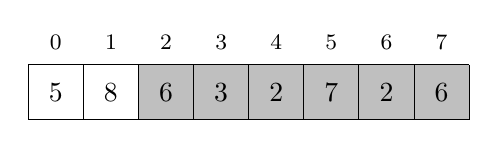
\begin{tikzpicture}[scale=0.7]
\fill[color=gray!50] (2,0) rectangle (8,1);
\draw (0,0) grid (8,1);

\node[anchor=center] at (0.5, 0.5) {5};
\node[anchor=center] at (1.5, 0.5) {8};
\node[anchor=center] at (2.5, 0.5) {6};
\node[anchor=center] at (3.5, 0.5) {3};
\node[anchor=center] at (4.5, 0.5) {2};
\node[anchor=center] at (5.5, 0.5) {7};
\node[anchor=center] at (6.5, 0.5) {2};
\node[anchor=center] at (7.5, 0.5) {6};

\footnotesize
\node at (0.5,1.4) {$0$};
\node at (1.5,1.4) {$1$};
\node at (2.5,1.4) {$2$};
\node at (3.5,1.4) {$3$};
\node at (4.5,1.4) {$4$};
\node at (5.5,1.4) {$5$};
\node at (6.5,1.4) {$6$};
\node at (7.5,1.4) {$7$};
\end{tikzpicture}
\end{center}
Here $\texttt{sum}_q(2,7)=6+3+2+7+2+6=26$.
In this case, the following two tree nodes
correspond to the range:
\begin{center}
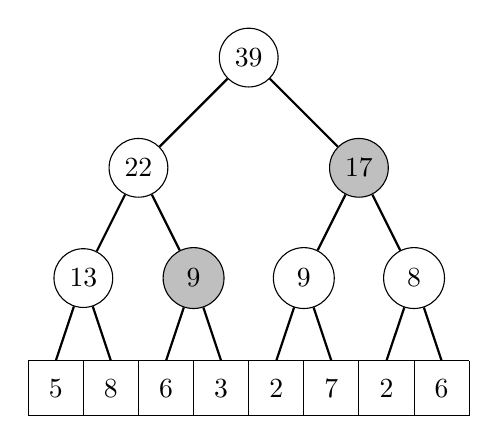
\begin{tikzpicture}[scale=0.7]
\draw (0,0) grid (8,1);

\node[anchor=center] at (0.5, 0.5) {5};
\node[anchor=center] at (1.5, 0.5) {8};
\node[anchor=center] at (2.5, 0.5) {6};
\node[anchor=center] at (3.5, 0.5) {3};
\node[anchor=center] at (4.5, 0.5) {2};
\node[anchor=center] at (5.5, 0.5) {7};
\node[anchor=center] at (6.5, 0.5) {2};
\node[anchor=center] at (7.5, 0.5) {6};

\node[draw, circle] (a) at (1,2.5) {13};
\path[draw,thick,-] (a) -- (0.5,1);
\path[draw,thick,-] (a) -- (1.5,1);
\node[draw, circle,fill=gray!50,minimum size=22pt] (b) at (3,2.5) {9};
\path[draw,thick,-] (b) -- (2.5,1);
\path[draw,thick,-] (b) -- (3.5,1);
\node[draw, circle,minimum size=22pt] (c) at (5,2.5) {9};
\path[draw,thick,-] (c) -- (4.5,1);
\path[draw,thick,-] (c) -- (5.5,1);
\node[draw, circle,minimum size=22pt] (d) at (7,2.5) {8};
\path[draw,thick,-] (d) -- (6.5,1);
\path[draw,thick,-] (d) -- (7.5,1);

\node[draw, circle] (i) at (2,4.5) {22};
\path[draw,thick,-] (i) -- (a);
\path[draw,thick,-] (i) -- (b);
\node[draw, circle,fill=gray!50] (j) at (6,4.5) {17};
\path[draw,thick,-] (j) -- (c);
\path[draw,thick,-] (j) -- (d);

\node[draw, circle] (m) at (4,6.5) {39};
\path[draw,thick,-] (m) -- (i);
\path[draw,thick,-] (m) -- (j);
\end{tikzpicture}
\end{center}
Thus, another way to calculate the sum is $9+17=26$.

When the sum is calculated using nodes
located as high as possible in the tree,
at most two nodes on each level
of the tree are needed.
Hence, the total number of nodes
is $O(\log n)$.

After an array update,
we should update all nodes
whose value depends on the updated value.
This can be done by traversing the path
from the updated array element to the top node
and updating the nodes along the path.

The following picture shows which tree nodes
change if the array value 7 changes:

\begin{center}
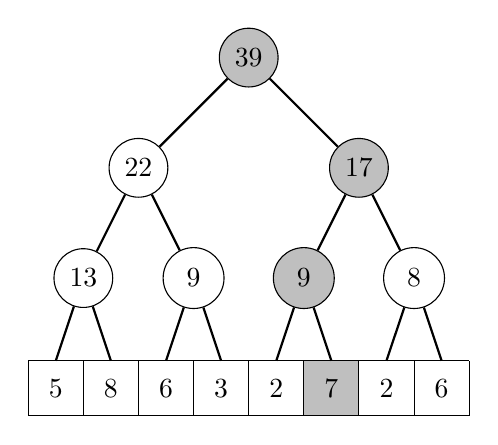
\begin{tikzpicture}[scale=0.7]
\fill[color=gray!50] (5,0) rectangle (6,1);
\draw (0,0) grid (8,1);

\node[anchor=center] at (0.5, 0.5) {5};
\node[anchor=center] at (1.5, 0.5) {8};
\node[anchor=center] at (2.5, 0.5) {6};
\node[anchor=center] at (3.5, 0.5) {3};
\node[anchor=center] at (4.5, 0.5) {2};
\node[anchor=center] at (5.5, 0.5) {7};
\node[anchor=center] at (6.5, 0.5) {2};
\node[anchor=center] at (7.5, 0.5) {6};

\node[draw, circle] (a) at (1,2.5) {13};
\path[draw,thick,-] (a) -- (0.5,1);
\path[draw,thick,-] (a) -- (1.5,1);
\node[draw, circle,minimum size=22pt] (b) at (3,2.5) {9};
\path[draw,thick,-] (b) -- (2.5,1);
\path[draw,thick,-] (b) -- (3.5,1);
\node[draw, circle,minimum size=22pt,fill=gray!50] (c) at (5,2.5) {9};
\path[draw,thick,-] (c) -- (4.5,1);
\path[draw,thick,-] (c) -- (5.5,1);
\node[draw, circle,minimum size=22pt] (d) at (7,2.5) {8};
\path[draw,thick,-] (d) -- (6.5,1);
\path[draw,thick,-] (d) -- (7.5,1);

\node[draw, circle] (i) at (2,4.5) {22};
\path[draw,thick,-] (i) -- (a);
\path[draw,thick,-] (i) -- (b);
\node[draw, circle,fill=gray!50] (j) at (6,4.5) {17};
\path[draw,thick,-] (j) -- (c);
\path[draw,thick,-] (j) -- (d);

\node[draw, circle,fill=gray!50] (m) at (4,6.5) {39};
\path[draw,thick,-] (m) -- (i);
\path[draw,thick,-] (m) -- (j);
\end{tikzpicture}
\end{center}

The path from bottom to top
always consists of $O(\log n)$ nodes,
so each update changes $O(\log n)$ nodes in the tree.

\subsubsection{Implementation}

We store a segment tree as an array
of $2n$ elements where $n$ is the size of
the original array and a power of two.
The tree nodes are stored from top to bottom:
$\texttt{tree}[1]$ is the top node,
$\texttt{tree}[2]$ and $\texttt{tree}[3]$
are its children, and so on.
Finally, the values from $\texttt{tree}[n]$
to $\texttt{tree}[2n-1]$ correspond to
the values of the original array
on the bottom level of the tree.

For example, the segment tree
\begin{center}
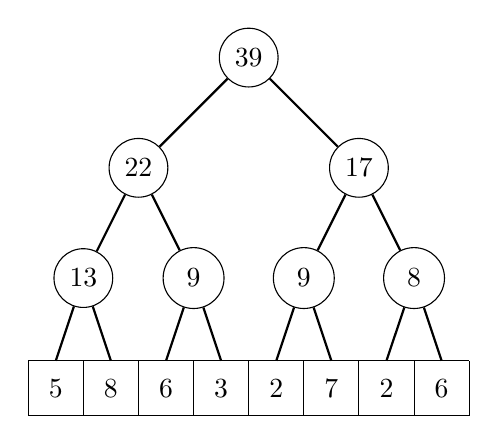
\begin{tikzpicture}[scale=0.7]
\draw (0,0) grid (8,1);

\node[anchor=center] at (0.5, 0.5) {5};
\node[anchor=center] at (1.5, 0.5) {8};
\node[anchor=center] at (2.5, 0.5) {6};
\node[anchor=center] at (3.5, 0.5) {3};
\node[anchor=center] at (4.5, 0.5) {2};
\node[anchor=center] at (5.5, 0.5) {7};
\node[anchor=center] at (6.5, 0.5) {2};
\node[anchor=center] at (7.5, 0.5) {6};

\node[draw, circle] (a) at (1,2.5) {13};
\path[draw,thick,-] (a) -- (0.5,1);
\path[draw,thick,-] (a) -- (1.5,1);
\node[draw, circle,minimum size=22pt] (b) at (3,2.5) {9};
\path[draw,thick,-] (b) -- (2.5,1);
\path[draw,thick,-] (b) -- (3.5,1);
\node[draw, circle,minimum size=22pt] (c) at (5,2.5) {9};
\path[draw,thick,-] (c) -- (4.5,1);
\path[draw,thick,-] (c) -- (5.5,1);
\node[draw, circle,minimum size=22pt] (d) at (7,2.5) {8};
\path[draw,thick,-] (d) -- (6.5,1);
\path[draw,thick,-] (d) -- (7.5,1);

\node[draw, circle] (i) at (2,4.5) {22};
\path[draw,thick,-] (i) -- (a);
\path[draw,thick,-] (i) -- (b);
\node[draw, circle] (j) at (6,4.5) {17};
\path[draw,thick,-] (j) -- (c);
\path[draw,thick,-] (j) -- (d);

\node[draw, circle] (m) at (4,6.5) {39};
\path[draw,thick,-] (m) -- (i);
\path[draw,thick,-] (m) -- (j);
\end{tikzpicture}
\end{center}
is stored as follows:
\begin{center}
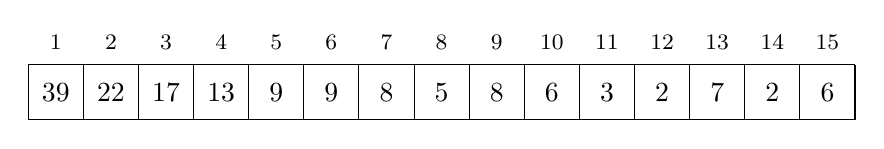
\begin{tikzpicture}[scale=0.7]
\draw (0,0) grid (15,1);

\node at (0.5,0.5) {$39$};
\node at (1.5,0.5) {$22$};
\node at (2.5,0.5) {$17$};
\node at (3.5,0.5) {$13$};
\node at (4.5,0.5) {$9$};
\node at (5.5,0.5) {$9$};
\node at (6.5,0.5) {$8$};
\node at (7.5,0.5) {$5$};
\node at (8.5,0.5) {$8$};
\node at (9.5,0.5) {$6$};
\node at (10.5,0.5) {$3$};
\node at (11.5,0.5) {$2$};
\node at (12.5,0.5) {$7$};
\node at (13.5,0.5) {$2$};
\node at (14.5,0.5) {$6$};

\footnotesize
\node at (0.5,1.4) {$1$};
\node at (1.5,1.4) {$2$};
\node at (2.5,1.4) {$3$};
\node at (3.5,1.4) {$4$};
\node at (4.5,1.4) {$5$};
\node at (5.5,1.4) {$6$};
\node at (6.5,1.4) {$7$};
\node at (7.5,1.4) {$8$};
\node at (8.5,1.4) {$9$};
\node at (9.5,1.4) {$10$};
\node at (10.5,1.4) {$11$};
\node at (11.5,1.4) {$12$};
\node at (12.5,1.4) {$13$};
\node at (13.5,1.4) {$14$};
\node at (14.5,1.4) {$15$};
\end{tikzpicture}
\end{center}
Using this representation,
the parent of $\texttt{tree}[k]$
is $\texttt{tree}[\lfloor k/2 \rfloor]$,
and its children are $\texttt{tree}[2k]$
and $\texttt{tree}[2k+1]$.
Note that this implies that the position of a node
is even if it is a left child and odd if it is a right child.

The following function
calculates the value of $\texttt{sum}_q(a,b)$:
\begin{lstlisting}
int sum(int a, int b) {
    a += n; b += n;
    int s = 0;
    while (a <= b) {
        if (a%2 == 1) s += tree[a++];
        if (b%2 == 0) s += tree[b--];
        a /= 2; b /= 2;
    }
    return s;
}
\end{lstlisting}
The function maintains a range
that is initially $[a+n,b+n]$.
Then, at each step, the range is moved
one level higher in the tree,
and before that, the values of the nodes that do not
belong to the higher range are added to the sum.

The following function increases the array value
at position $k$ by $x$:
\begin{lstlisting}
void add(int k, int x) {
    k += n;
    tree[k] += x;
    for (k /= 2; k >= 1; k /= 2) {
        tree[k] = tree[2*k]+tree[2*k+1];
    }
}
\end{lstlisting}
First the function updates the value
at the bottom level of the tree.
After this, the function updates the values of all
internal tree nodes, until it reaches
the top node of the tree.

Both the above functions work
in $O(\log n)$ time, because a segment tree
of $n$ elements consists of $O(\log n)$ levels,
and the functions move one level higher
in the tree at each step.

\subsubsection{Other queries}

Segment trees can support all range queries
where it is possible to divide a range into two parts,
calculate the answer separately for both parts
and then efficiently combine the answers.
Examples of such queries are
minimum and maximum, greatest common divisor,
and bit operations and, or and xor.

For example, the following segment tree
supports minimum queries:

\begin{center}
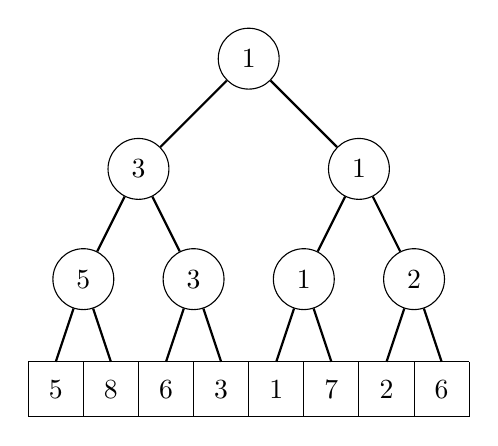
\begin{tikzpicture}[scale=0.7]
\draw (0,0) grid (8,1);

\node[anchor=center] at (0.5, 0.5) {5};
\node[anchor=center] at (1.5, 0.5) {8};
\node[anchor=center] at (2.5, 0.5) {6};
\node[anchor=center] at (3.5, 0.5) {3};
\node[anchor=center] at (4.5, 0.5) {1};
\node[anchor=center] at (5.5, 0.5) {7};
\node[anchor=center] at (6.5, 0.5) {2};
\node[anchor=center] at (7.5, 0.5) {6};

\node[draw, circle,minimum size=22pt] (a) at (1,2.5) {5};
\path[draw,thick,-] (a) -- (0.5,1);
\path[draw,thick,-] (a) -- (1.5,1);
\node[draw, circle,minimum size=22pt] (b) at (3,2.5) {3};
\path[draw,thick,-] (b) -- (2.5,1);
\path[draw,thick,-] (b) -- (3.5,1);
\node[draw, circle,minimum size=22pt] (c) at (5,2.5) {1};
\path[draw,thick,-] (c) -- (4.5,1);
\path[draw,thick,-] (c) -- (5.5,1);
\node[draw, circle,minimum size=22pt] (d) at (7,2.5) {2};
\path[draw,thick,-] (d) -- (6.5,1);
\path[draw,thick,-] (d) -- (7.5,1);

\node[draw, circle,minimum size=22pt] (i) at (2,4.5) {3};
\path[draw,thick,-] (i) -- (a);
\path[draw,thick,-] (i) -- (b);
\node[draw, circle,minimum size=22pt] (j) at (6,4.5) {1};
\path[draw,thick,-] (j) -- (c);
\path[draw,thick,-] (j) -- (d);

\node[draw, circle,minimum size=22pt] (m) at (4,6.5) {1};
\path[draw,thick,-] (m) -- (i);
\path[draw,thick,-] (m) -- (j);
\end{tikzpicture}
\end{center}

In this case, every tree node contains
the smallest value in the corresponding
array range.
The top node of the tree contains the smallest
value in the whole array.
The operations can be implemented like previously,
but instead of sums, minima are calculated.

The structure of a segment tree also allows us
to use binary search for locating array elements.
For example, if the tree supports minimum queries,
we can find the position of an element
with the smallest value in $O(\log n)$ time.

For example, in the above tree, an
element with the smallest value 1 can be found
by traversing a path downwards from the top node:

\begin{center}
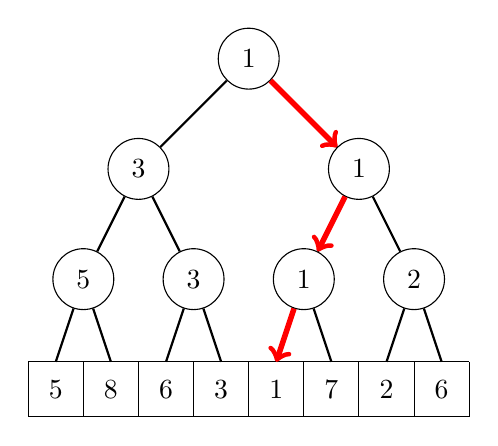
\begin{tikzpicture}[scale=0.7]
\draw (0,0) grid (8,1);

\node[anchor=center] at (0.5, 0.5) {5};
\node[anchor=center] at (1.5, 0.5) {8};
\node[anchor=center] at (2.5, 0.5) {6};
\node[anchor=center] at (3.5, 0.5) {3};
\node[anchor=center] at (4.5, 0.5) {1};
\node[anchor=center] at (5.5, 0.5) {7};
\node[anchor=center] at (6.5, 0.5) {2};
\node[anchor=center] at (7.5, 0.5) {6};

\node[draw, circle,minimum size=22pt] (a) at (1,2.5) {5};
\path[draw,thick,-] (a) -- (0.5,1);
\path[draw,thick,-] (a) -- (1.5,1);
\node[draw, circle,minimum size=22pt] (b) at (3,2.5) {3};
\path[draw,thick,-] (b) -- (2.5,1);
\path[draw,thick,-] (b) -- (3.5,1);
\node[draw, circle,minimum size=22pt] (c) at (5,2.5) {1};
\path[draw,thick,-] (c) -- (4.5,1);
\path[draw,thick,-] (c) -- (5.5,1);
\node[draw, circle,minimum size=22pt] (d) at (7,2.5) {2};
\path[draw,thick,-] (d) -- (6.5,1);
\path[draw,thick,-] (d) -- (7.5,1);

\node[draw, circle,minimum size=22pt] (i) at (2,4.5) {3};
\path[draw,thick,-] (i) -- (a);
\path[draw,thick,-] (i) -- (b);
\node[draw, circle,minimum size=22pt] (j) at (6,4.5) {1};
\path[draw,thick,-] (j) -- (c);
\path[draw,thick,-] (j) -- (d);

\node[draw, circle,minimum size=22pt] (m) at (4,6.5) {1};
\path[draw,thick,-] (m) -- (i);
\path[draw,thick,-] (m) -- (j);

\path[draw=red,thick,->,line width=2pt] (m) -- (j);
\path[draw=red,thick,->,line width=2pt] (j) -- (c);
\path[draw=red,thick,->,line width=2pt] (c) -- (4.5,1);
\end{tikzpicture}
\end{center}

\section{Additional techniques}

\subsubsection{Index compression}

A limitation in data structures that
are built upon an array is that
the elements are indexed using
consecutive integers.
Difficulties arise when large indices
are needed.
For example, if we wish to use the index $10^9$,
the array should contain $10^9$
elements which would require too much memory.

\index{index compression}

However, we can often bypass this limitation
by using \key{index compression},
where the original indices are replaced
with indices $1,2,3,$ etc.
This can be done if we know all the indices
needed during the algorithm beforehand.

The idea is to replace each original index $x$
with $c(x)$ where $c$ is a function that
compresses the indices.
We require that the order of the indices
does not change, so if $a<b$, then $c(a)<c(b)$.
This allows us to conveniently perform queries
even if the indices are compressed.

For example, if the original indices are
$555$, $10^9$ and $8$, the new indices are:

\[
\begin{array}{lcl}
c(8) & = & 1 \\
c(555) & = & 2 \\
c(10^9) & = & 3 \\
\end{array}
\]

\subsubsection{Range updates}

So far, we have implemented data structures
that support range queries and updates
of single values.
Let us now consider an opposite situation,
where we should update ranges and
retrieve single values.
We focus on an operation that increases all
elements in a range $[a,b]$ by $x$.

\index{difference array}

Surprisingly, we can use the data structures
presented in this chapter also in this situation.
To do this, we build a \key{difference array}
whose values indicate
the differences between consecutive values
in the original array.
Thus, the original array is the
prefix sum array of the
difference array.
For example, consider the following array:

\begin{center}
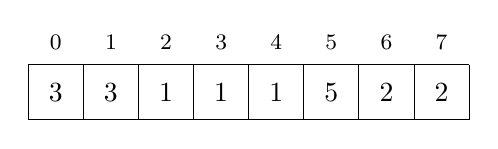
\begin{tikzpicture}[scale=0.7]
\draw (0,0) grid (8,1);

\node at (0.5,0.5) {$3$};
\node at (1.5,0.5) {$3$};
\node at (2.5,0.5) {$1$};
\node at (3.5,0.5) {$1$};
\node at (4.5,0.5) {$1$};
\node at (5.5,0.5) {$5$};
\node at (6.5,0.5) {$2$};
\node at (7.5,0.5) {$2$};


\footnotesize
\node at (0.5,1.4) {$0$};
\node at (1.5,1.4) {$1$};
\node at (2.5,1.4) {$2$};
\node at (3.5,1.4) {$3$};
\node at (4.5,1.4) {$4$};
\node at (5.5,1.4) {$5$};
\node at (6.5,1.4) {$6$};
\node at (7.5,1.4) {$7$};
\end{tikzpicture}
\end{center}

The difference array for the above array is as follows:
\begin{center}
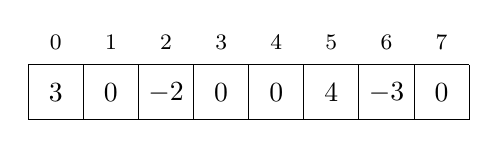
\begin{tikzpicture}[scale=0.7]
\draw (0,0) grid (8,1);

\node at (0.5,0.5) {$3$};
\node at (1.5,0.5) {$0$};
\node at (2.5,0.5) {$-2$};
\node at (3.5,0.5) {$0$};
\node at (4.5,0.5) {$0$};
\node at (5.5,0.5) {$4$};
\node at (6.5,0.5) {$-3$};
\node at (7.5,0.5) {$0$};


\footnotesize
\node at (0.5,1.4) {$0$};
\node at (1.5,1.4) {$1$};
\node at (2.5,1.4) {$2$};
\node at (3.5,1.4) {$3$};
\node at (4.5,1.4) {$4$};
\node at (5.5,1.4) {$5$};
\node at (6.5,1.4) {$6$};
\node at (7.5,1.4) {$7$};
\end{tikzpicture}
\end{center}

For example, the value 2 at position 6 in the original array
corresponds to the sum $3-2+4-3=2$ in the difference array.

The advantage of the difference array is
that we can update a range
in the original array by changing just
two elements in the difference array.
For example, if we want to 
increase the original array 
values between positions 1 and 4 by 5,
it suffices to increase the
difference array value at position 1 by 5
and decrease the value at position 5 by 5.
The result is as follows:

\begin{center}
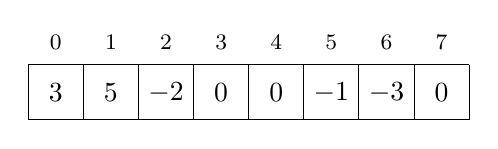
\begin{tikzpicture}[scale=0.7]
\draw (0,0) grid (8,1);

\node at (0.5,0.5) {$3$};
\node at (1.5,0.5) {$5$};
\node at (2.5,0.5) {$-2$};
\node at (3.5,0.5) {$0$};
\node at (4.5,0.5) {$0$};
\node at (5.5,0.5) {$-1$};
\node at (6.5,0.5) {$-3$};
\node at (7.5,0.5) {$0$};

\footnotesize
\node at (0.5,1.4) {$0$};
\node at (1.5,1.4) {$1$};
\node at (2.5,1.4) {$2$};
\node at (3.5,1.4) {$3$};
\node at (4.5,1.4) {$4$};
\node at (5.5,1.4) {$5$};
\node at (6.5,1.4) {$6$};
\node at (7.5,1.4) {$7$};
\end{tikzpicture}
\end{center}

More generally, to increase the values
in range $[a,b]$ by $x$,
we increase the value at position $a$ by $x$
and decrease the value at position $b+1$ by $x$.
Thus, it is only needed to update single values
and process sum queries,
so we can use a binary indexed tree or a segment tree.

A more difficult problem is to support both
range queries and range updates.
In Chapter 28 we will see that even this is possible.



